\subsection*{Wykresy fazowe}
Są to wykresy zależności ciśnienia od temperatury, przy danej temperaturze i~ciśnieniu można odczytać fazę. Prezentują nie tylko zmiany stanu skupienia, ale także np. zmianę struktury krystalicznej.
\begin{mathfigure*}
    \drawaxes{0, 0}{3, 3}[\(T\)][\(p\)];
    \draw[domain=0:1, thick, blue] plot (\x, {\x * \x});
    \draw[domain=1:2.3, thick, red] plot (\x, {(\x - 1) * (\x - 1) + 1});
    \draw[domain=0.6:1, thick, Green] plot (\x, {9 * (\x - 1) * (\x - 1) + 1});
    \fillpoint*{2.3, 2.69}[punkt krytyczny][right];
    \fillpoint*{1, 1}[punkt potrójny][right];
    \node at (1.5, 0) [above]{gaz};
    \node at (0.7, 1.7) [right]{ciecz};
    \path (0, 3) -- node[pos=0.6, sloped, above]{ciało stałe} (0, 0);
\end{mathfigure*}
Punkt potrójny --- warunki, w~których ciało jest w~równowadze pomiędzy wszystkimi fazami, żadna faza nie zwiększa swojej ilości. Punkt potrójny dla wody:
\begin{description}
    \item \(T = 273,16\K\)
    \item \(p = 611\Pa\)
\end{description}
Punkt krytyczny --- punkt, w~którym wykres się urywa --- powyżej tego punktu substancja występuje tylko w~postaci gazowej (para) niezależnie od ciśnienia. Punkt krytyczny dla wody:
\begin{description}
    \item \(T = 674,2\K\)
    \item \(p = 22,1\Mega\Pa\)
\end{description}
\subsubsection*{Własności gazu i~pary nasyconej}
W~przemianie izotermicznej \(T = \constfont{const}\):
\begin{figure}[h!]
    \centering
    \begin{tikzpicture}
        \drawaxes{0, 0}{3, 3}[\(V\)][\(p\)];
        \draw[domain=0.5:2.5] plot (\x, {1/\x});
        \node at (1.5, 3.5) {gaz};
    \end{tikzpicture}
    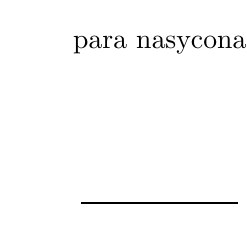
\begin{tikzpicture}
        \drawaxes{0, 0}{3, 3}[\(V\)][\(p\)];
        \draw[domain=0.5:2.5] plot (\x, 1.5);
        \node at (1.5, 3.5) {para nasycona};
    \end{tikzpicture}
\end{figure}\\
W~przemianie izochorycznej \(V = \constfont{const}\):
\begin{figure}[h!]
    \centering
    \begin{tikzpicture}
        \drawaxes{0, 0}{3, 3}[\(T\)][\(p\)];
        \draw[domain=0.5:2.5] plot (\x, {0.8 * \x});
        \draw[dotted, domain=0:0.5] plot (\x, {0.8 * \x});
        \node at (1.5, 3.5) {gaz};
    \end{tikzpicture}
    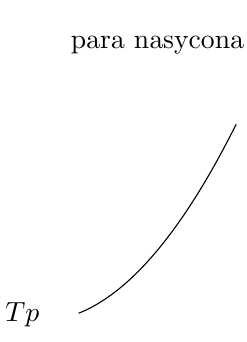
\begin{tikzpicture}
        \drawaxes{0, 0}{3, 3}[\(T\)][\(p\)];
        \draw[domain=0.5:2.5] plot (\x, {0.4 * \x * \x});
        \node at (1.5, 3.5) {para nasycona};
    \end{tikzpicture}
\end{figure}
\subsubsection*{Jak wyznaczyć temperaturę krytyczną gazu?}
Zaczynamy od izotermy, następnie obniżamy temperaturę i~obserwujemy wykres \(p(V)\). Im bardziej obniżamy temperaturę, tym dłuższe fragmenty stałe pojawiają się w~hiperboli. Teraz prowadzimy parabolę przez punkty końcowe fragmentów stałych. W~wierzchołku tej paraboli jest temperatura krytyczna.
\subsubsection*{Skraplanie gazu}
Np. dla tlenu temperatura krytyczna wynosi \(T_k = 154,6\K\). Dlatego był problem ze skropleniem tlenu, ponieważ jeśli nie zejdziemy ponieżej temperatury krytycznej, nie ma szans skroplić gazu. Karol Olszewski i~Zygmunt Wróblewski na UJ po raz pierwszy w~historii skroplili tlen. Zrobili to metodą kaskadową:
\begin{enumerate}
    \item skraplamy gaz, który ma nieco wyższą temperaturę krytyczną niż gaz docelowy. W~zbiorniku powstaje ciecz, a~nad nią para
    \item następnie dodajemy kolejny gaz o~nieco niższej temperaturze krytycznej, on się skrapla i~powtarzamy proces
\end{enumerate}
\subsubsection*{Inne informacje}
\begin{itemize}
    \item azot intensywnie paruje, więc potem zostaje prawie sam ciekły tlen
\end{itemize}
\subsubsection*{Wcale nie zadanie wcale nie domowe}
Research:
\begin{itemize}
    \item punkt potrójny wody i~dwutlenku węgla --- jakie zjawiska, jakie warunki?
    \item nadciekłość helu --- jakie zjawiska, jakie dziwne własności?
\end{itemize}
